\documentclass{ctexart}
\usepackage[T1]{fontenc}
\usepackage[a4paper,top=1.5cm,bottom=1.5cm,left=2cm,right=2cm,marginparwidth=1.75cm]{geometry}
\usepackage{mathtools}
\usepackage{tikz}
\usepackage{booktabs}
\usepackage{caption}
\usepackage{outlines}
\usepackage{graphicx}
\usepackage{float}
\usepackage{amsthm}
\usepackage{tabularray}
\usepackage{minted}
\usepackage[colorlinks=false, allcolors=blue]{hyperref}
\usepackage{cleveref}
\renewcommand{\tableautorefname}{表}
\UseTblrLibrary{booktabs}
\DeclarePairedDelimiter{\set}{\{}{\}}
\DeclarePairedDelimiter{\paren}{(}{)}
\graphicspath{ {./images/} }

\newcounter{fullrefcounter}
\newcommand*{\fullref}[1]{%
\addtocounter{fullrefcounter}{1}%
\label{--ref-\thefullrefcounter}%
\ifthenelse{\equal{\getpagerefnumber{--ref-\thefullrefcounter}}{\getpagerefnumber{#1}}}
  {
    \hyperref[{#1}]{\Cref*{#1} \nameref*{#1}}
  }
  {% false case
    \hyperref[{#1}]{第 \pageref*{#1} 页 \Cref*{#1} \nameref*{#1}}
  }
}

\title{编译原理第五次作业}
\author{卢雨轩 19071125}
% \date{\today}
\ctexset{
    section = {
        titleformat = \raggedright,
        name = {,},
        number = \chinese{section}、
    },
    paragraph = {
        runin = false
    },
    today = small,
    figurename = 图,
    contentsname = 目录,
    tablename = 表,
}

\begin{document}

\maketitle

\begin{outline}
    \1[12.] $G = \begin{cases}
        S \to aSSb \\
        S \to aSSS \\
        S \to c
    \end{cases}$
    \2[(1)]
    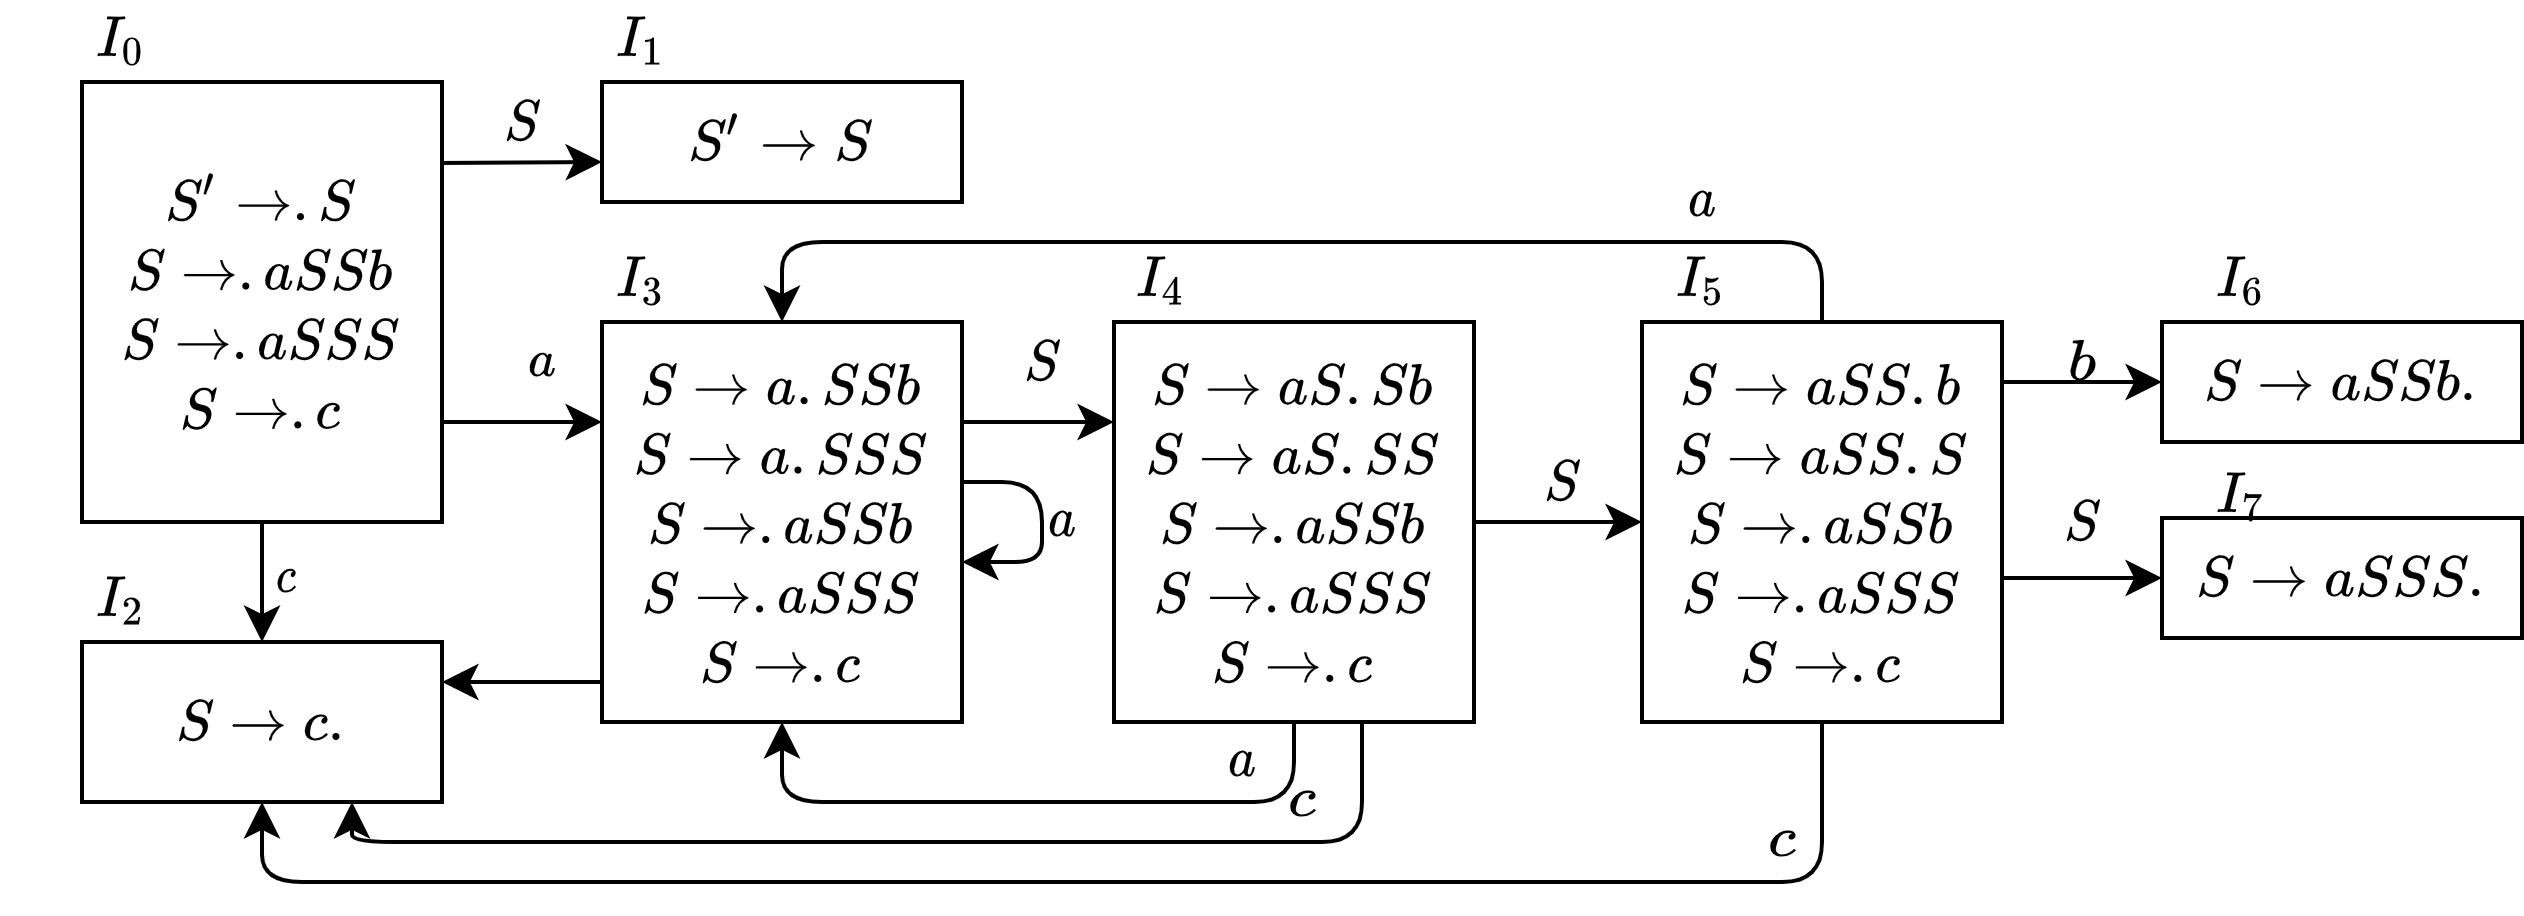
\includegraphics[width=\linewidth]{homework-5-0.drawio.png}
    \2[(2)]
    \begin{tblr}{}
        & \vline  a & b & c & \# &\vline S \\
        \hline 0 & S3 & & S2 & & 1 \\
        1 & & & & acc & \\
        2 & r3 & r3 & r3 & e3 & \\
        3 & S3 & & S2 & & 4 \\
        4 & S3 & & S2 & & 5 \\
        5 & S3 & S6 & S2 & & 7 \\
        6 & r1 & r1 & r1 & r1 \\
        7 & r2 & r2 & r2 & r2 \\
    \end{tblr}
    \1[13.] $G = \begin{cases}
        S \to 0S0 \\
        S \to 1S1 \\
        S \to 01
    \end{cases}$
        \2[(1)]
        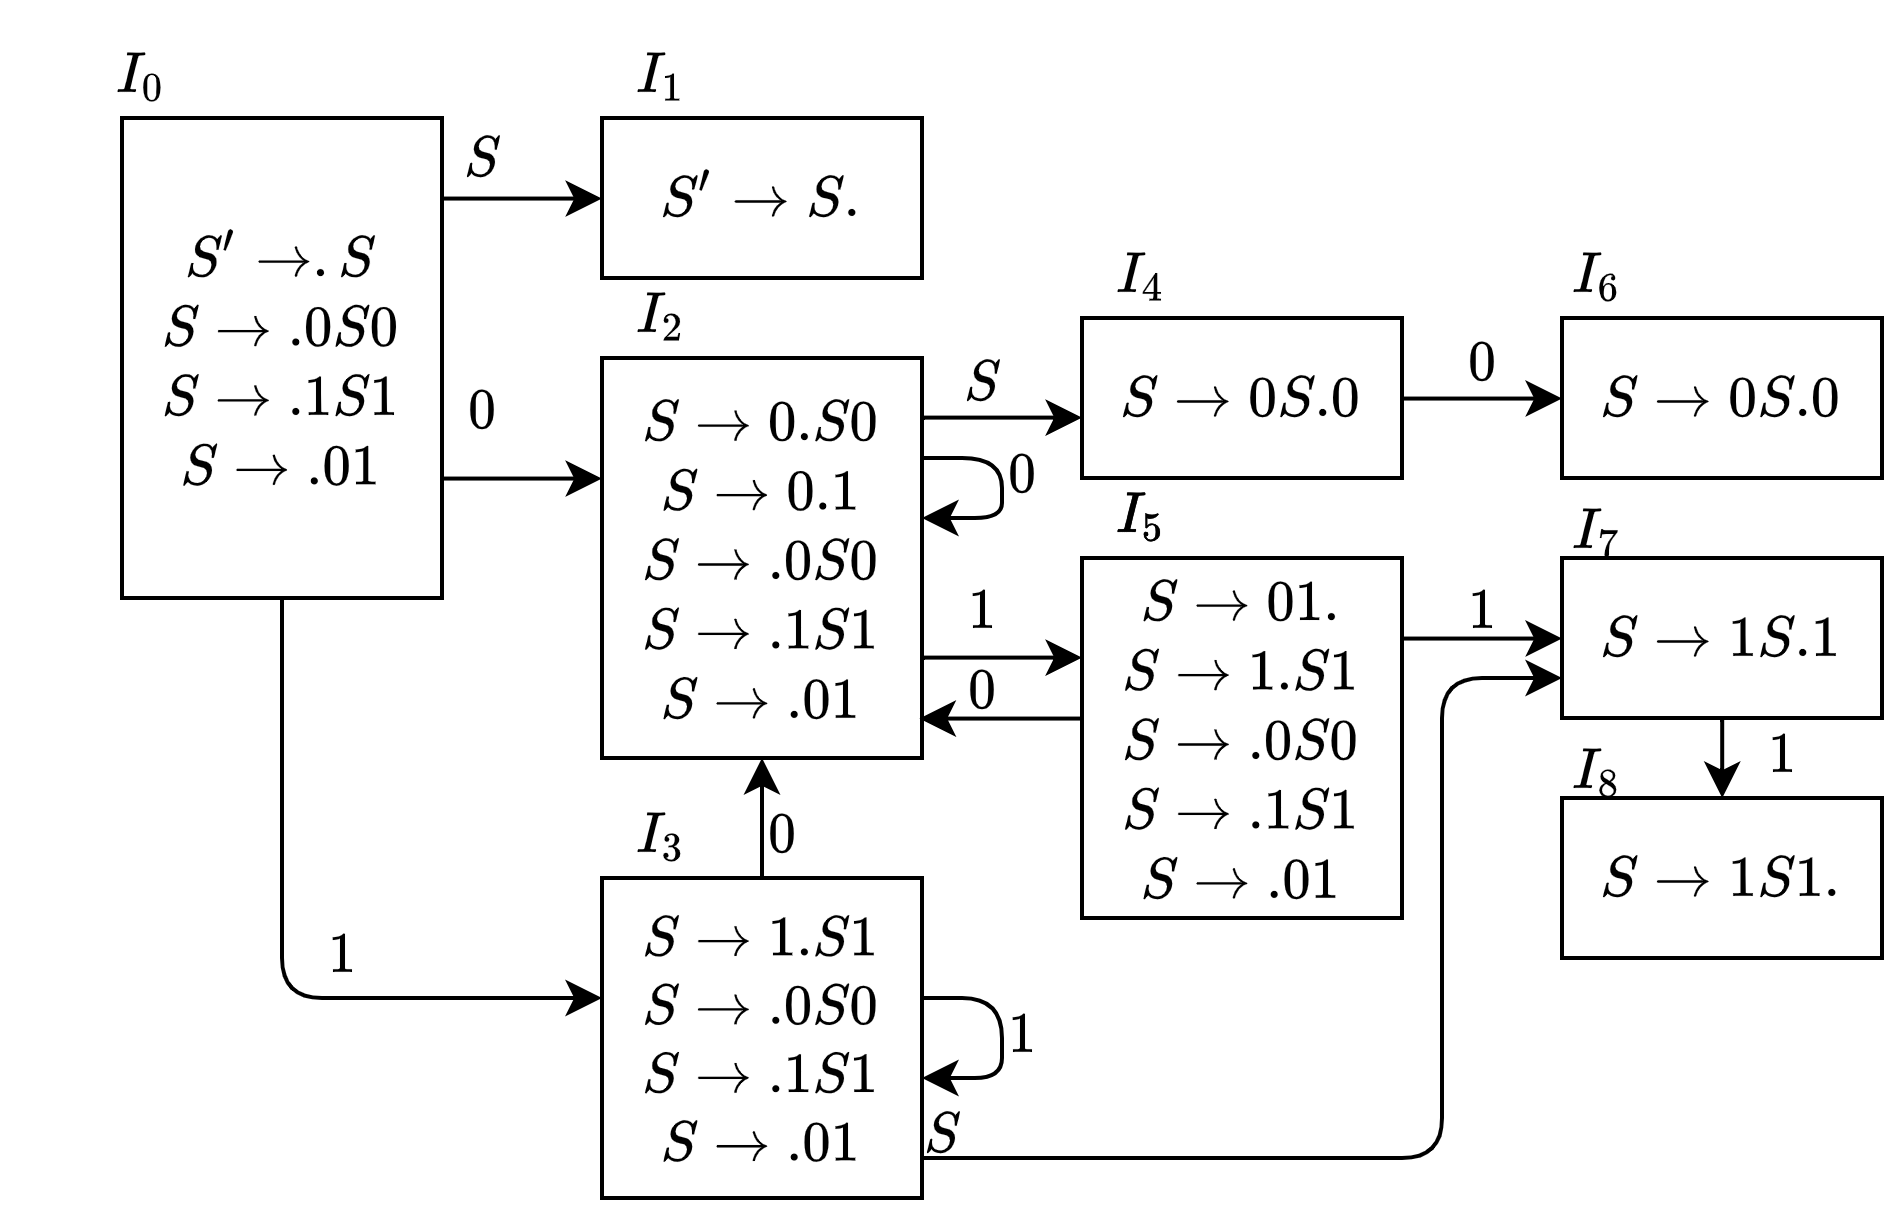
\includegraphics[width=\linewidth]{homework-5-1.drawio.png}
        \2[(2)] $I_5$ 中存在 移进-归约冲突。$FOLLOW(S) = \set{0, 1, \#}$,移进项目$S \to .1S1$中的首个符号在$FOLLOW(S)$中,因此均可进行。无法解决重提。
\end{outline}

\end{document}
